%!TEX root=main.tex
\section{The Cautious Adaptation Approach}

Given a component that does not satisfy the global requirements of a system, although it is necessary to use the component. We call this component {\em defiant} if it can still be modified by adapting the system wrapping around it. In general, when a self-adaptive system can have multiple components that need to be adapted to its global requirement, however, none of them alone can achieve this demand. In this section, we lay out a step-wise approach to address this problem (see an overview in Figure~\ref{fig:process}).

\subsection{Overview}

Our process to address a defiant component can be divided into three phases, as illustrated by Figure~\ref{fig:process}: (i) \textit{defiant component identification}, (ii) \textit{wrapper design and implementation}, and (iii) \textit{runtime cautious adaptation}. The first two phases occur at design time, while the last one occurs at run time. %Each phase is detailed as follows. 

\begin{figure*}[h]\centering
% 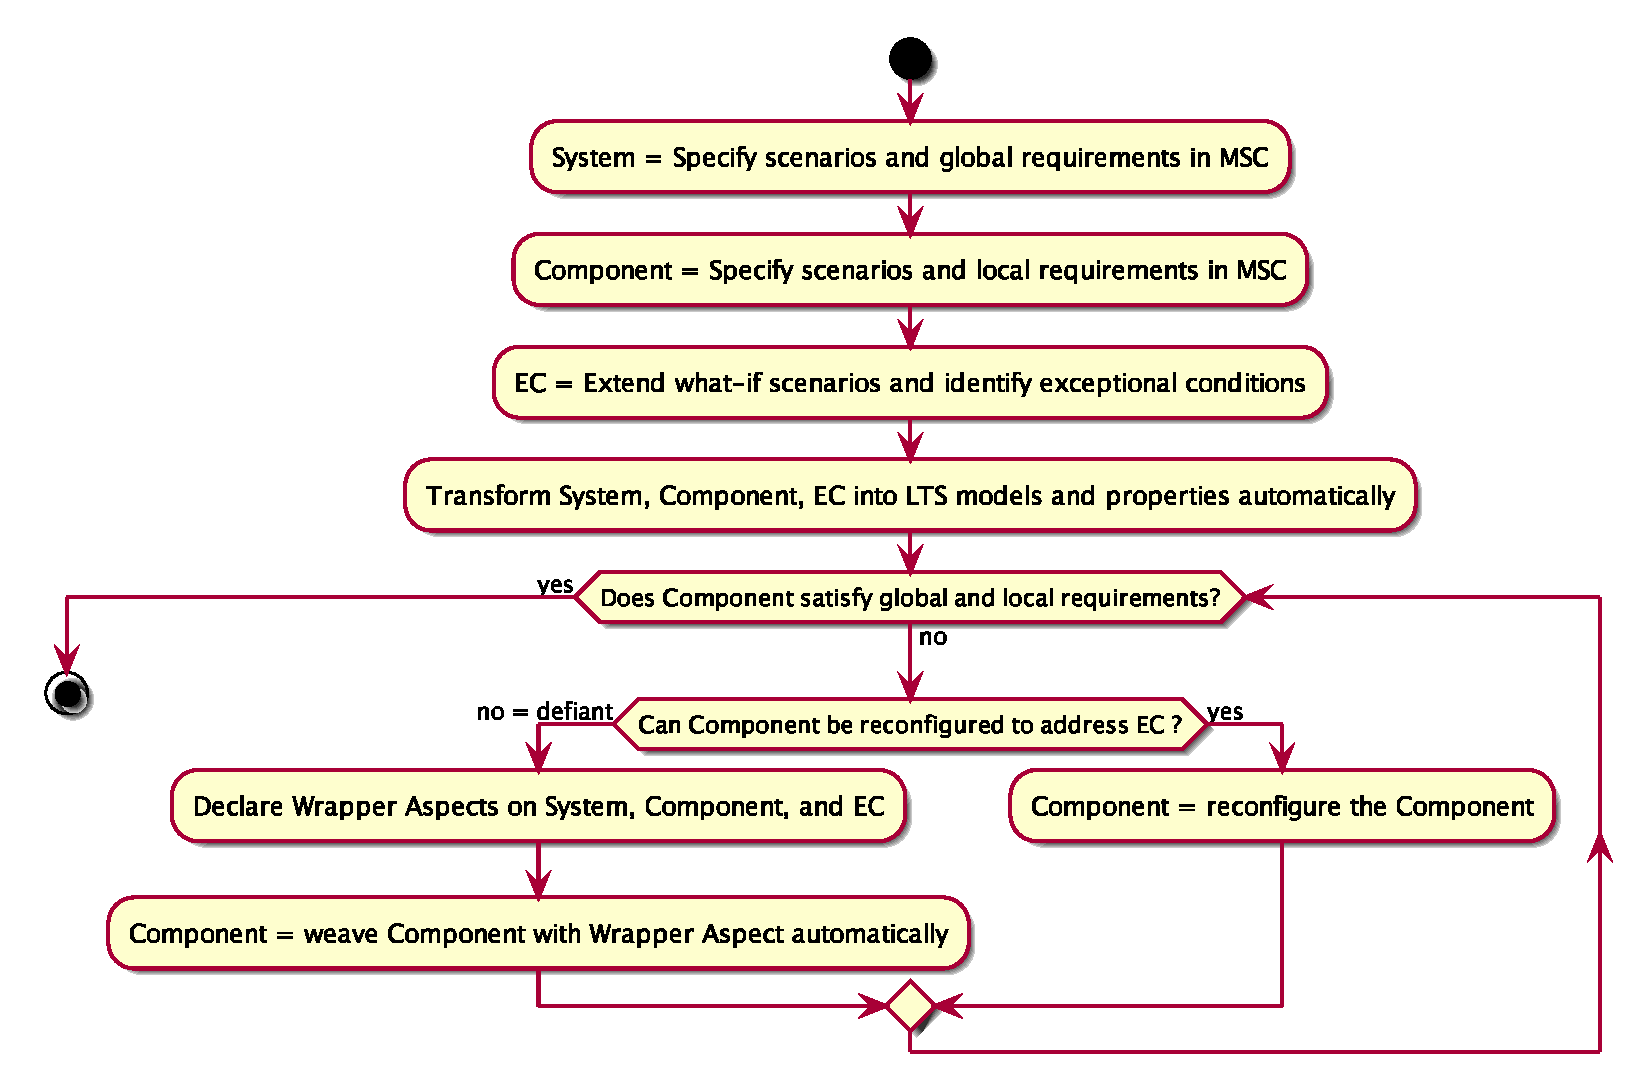
\includegraphics[width=0.9\columnwidth]{figures/activity.eps}
 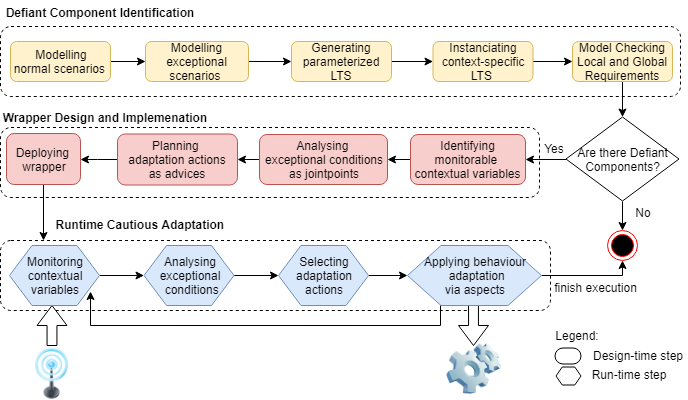
\includegraphics[width=0.8\textwidth]{figures/workflow2.png}
 \caption{Overview of the cautious adaptation approach in a workflow diagram}
 \label{fig:process}
 \vspace*{-0.5cm}
\end{figure*}

The first phase uses scenarios to model the system for formally verifying the defiant behaviour problems. In particular, we have chosen the Message Sequence Chart~\cite{harel2003} (MSC) specification, a standard International Telecommunication Union (ITU) notation for describing the interaction between communicating processes, to model both ordinary and exceptional scenarios. 

The ITU-T Recommendation Z.120 \cite{itu1994} specifies two main syntactic objects as components of the MSC notation: \textit{basic MSC} (bMSC) and \textit{high MSC} (HMSC). A bMSC consists of a set of processes (called instances in Z.120) that run in parallel and exchange messages in a one-to-one, asynchronous manner. A number of bMSCs may be connected in a directed graph to describe parallel, sequential, iterating, and non-deterministic execution. The resulting diagram is an HMSC, in which all nodes refer to bMSCs, and the edges indicate execution sequences possible along the nodes. %In addition, an HMSC can hierarchically describe a system by combining HMSCs within an HMSC. 
%Assuming that high-level message sequence charts (hMSC) and basic message sequence charts are used to model the defiant behaviour in the system.  

In the second phase the user implements and deploys the self-adaptive solution by addressing the steps of the MAPE-K loop using an aspect-oriented language. 

Finally, in the last phase the user deploys the self-adaptive solutions to incorporate sensors and actuators of the real system.

The second design-time phase to address the defiant behaviour previously identified aims at implementing the wrapper solution as an aspect. To do that, it includes four steps that encompasses the activities of the MAPE loop to design the wrapper solution, that is subsequently implemented using an AOP language. 


%\subsubsection{Runtime Cautious Adaptation}

In the final phase, the system weaved with the wrapper is executed. At runtime, it is now managed by a MAPE loop implemented by the aspect. During the execution, the contextual variables identified at the design-time must be observable directly or indirectly using dedicated sensors. If they are in place, appropriate interpretation of the readings need to be added to relate the observed behaviours with the monitored properties. When an exceptional condition is identified, the wrapper selects the appropriate action, that causes a system behaviour adaptation. 

To do that, the controls in the system need to be added to wrapper around the defiant components when necessary. With such wrapping, the input to the original component may need to be filtered so that, without internal changes to the component, the composed wrapper would satisfy the global requirements the original component is not aware of. 

Connecting the components and the wrapper together is the role of aspect execution engine, which not only ensure that the design-time model are faithfully executed at the runtime, but also potential conflicts between the wrappers of multiple defiant components are handled properly. 


%Therefore, the cautious adaptation approach involves designing a wrapper aspect, which is defined by a specification of the pointcuts and advices on the scenarios, and transforming them into LTS specifications by extending the previous work of scenario to LTS translation. After that, the LTS specifications of both the global context and the wrapped component will be used to check, formally, whether or not the adapted system satisfy the safety properties of both the global requirements in the exceptional conditions and the local requirements in the normal conditions.

%First, when an off-the-shelf component is used in an emergent global system, scenarios are specified with respect to the global and local requirements.By transforming these scenarios into LTS behaviour models, along with their requirements transformed into properties, we use model checker to tell whether the off-the-shelf component can satisfy the global requirements, which it was not designed for. Upon failure to satisfy the requirements, the designer can ask it to change its behaviour. However, resisting to the change request, the designer has to identify the component as a defiant component, and treat it cautiously.

%\subsection{Discussion about Self-Adaptation}

%Existing self-adaptive systems rely on a full monitoring-analysis-planning-execution (MAPE) feedback loop to continuously monitor the environment and switch to alternative solutions when the requirements are not satisfied. However, we observe that it is not always necessary to monitor the entire process. Given the prior knowledge of the environment, to reduce the monitoring and adaptation overhead, it is possible to monitor only part of the processes while switch to part of the solutions when the adaptation is required.  In this way, cautious adaption can be seen as a means towards more efficient self-adaptation.
% TODO. Can we evaluate the efficiency of self-adaptation by measuring the efficiency?


\subsection{Formalisation}

The general problem being tackled can be formalised using the semantics of Problem Frames~\cite{DBLP:books/daglib/0022946}, as follows. At the design time of a defiant component ($c$), given its world context ($W_c$), its specification ($S_c$) must satisfy its requirements ($R_c$), i.e., $W_c, S_c \models R_c$. 

%For instance, consider drone component $c$ with two requirements $R_c = R_1 \wedge R_2$, where $R_1$ is ``to fly from location $A$ to location $B$ when the battery level is above a threshold $\theta = 10\%$'' ($W_1$), and $R_2$ is ``to land safely when the battery level drops below $\theta$'' ($W_2 = \neg W_1$).

Suppose that component $c$ is being used as part of a system-of-systems ($s$). Based on the analysis of exception scenarios concerning a specific context of the system ($W_s$), which satisfies the condition $W_s \implies W_c$, component $c$ cannot satisfy global requirements of $s$. In other words, $W_s, S_s \not \models R_s$, where $S_s$ contains $S_c$. 

%In order to illustrate, consider the drone application scenario with an exceptional condition defined as $W_s = W_2 \wedge W_3 \wedge W_4$ where the battery level is below $\theta$ ($W_2$), but the battery level is sufficient to fly to location $B$ because of the wind condition ($W_3$), and it is flying above water by design of $S_s$ ($W_4$). According to the designed specification of the component $S_c$, the drone will land because of $W_2$, regardless of $W_3$, and the drone will land in the water because of $W_4$. The only feasible solution is to avoid safe landing in $W_s$, because if one rescues the landed drone from the water, it will be too late to replace it with another means of transportation even if the payload will not be damaged. Therefore, the problem is that it is not possible to change the specification of $S_c$. 

To verify that the wrapper executes its purpose, we formalise three conditions to be checked as follows:
\[
\begin{array}{ll}
W_s, S_s \not \models R_s & (\mbox{defiant identification})\\
W_s, S_s |_{c\rightarrow w(c)} \models R_s & (\mbox{defiant removal}) \\
W_c \setminus W_s, S_{w(c)} \models R_c & (\mbox{safety assurance})
\end{array}
\]
\begin{itemize}
\item Defiant identification checks that the component is defiant because its configurations do not satisfy global requirements.

\item Defiant removal checks that after wrapping up the defiant component with new behaviour, the global requirement can be restored in exceptional conditions.

\item Safety assurance checks that after wrapping up the defiant component with new behaviour, the local requirements are still satisfied in normal conditions. 
\end{itemize}

%\subsection{Scenario Extensions on MSC}

\subsection{Tool Support}
To support the method, we extend the message sequence chart (MSC) specification with a decision point  to represent an \textit{interception point} in which exceptional conditions can be added around the defiant component. 

Several exceptional conditions can be intercepting in the same decision point, indicating other possible behaviours according to alternative contexts. If there is no exceptional scenario plugged in an interception point, the expected default behaviour is performed.

%\begin{figure*}[h]\centering
% 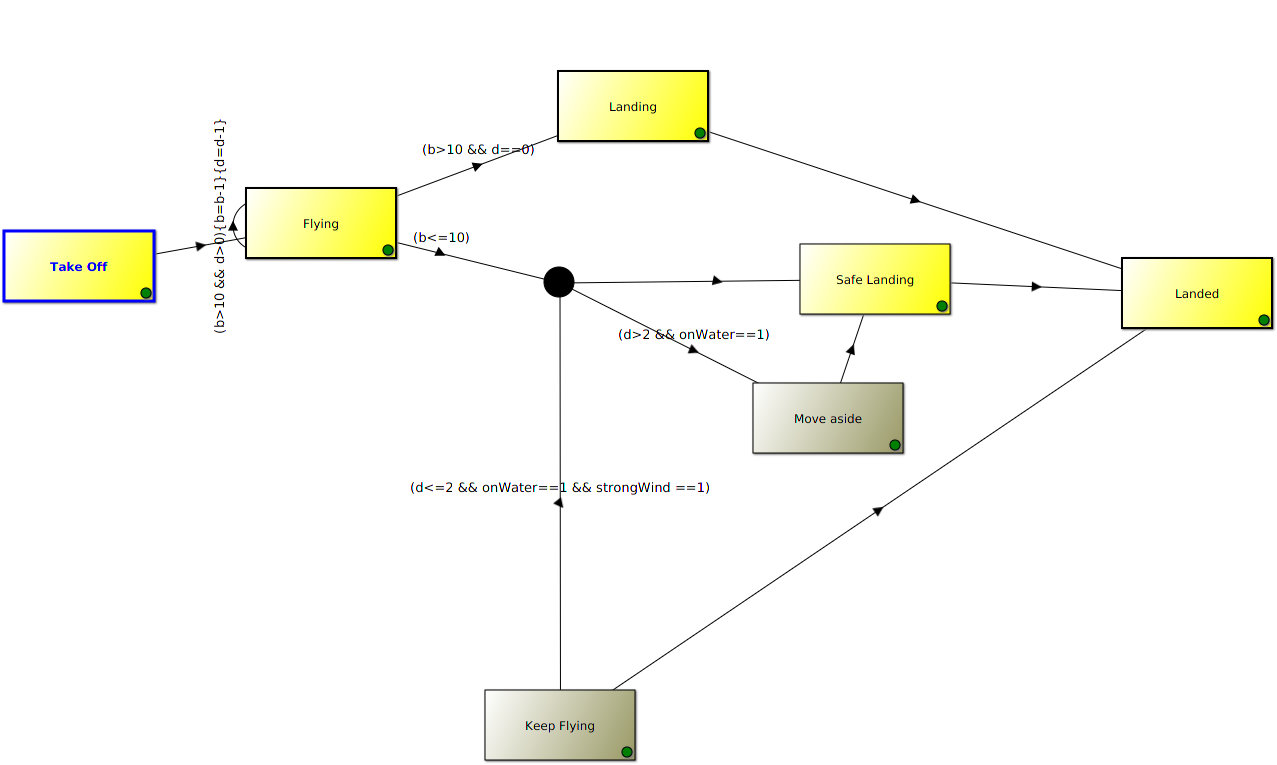
\includegraphics[width=0.8\textwidth]{figures/1-hMSC-Drone.png}
%    \caption{Extended hMSCs for the drone scenario. Each box defines a basic message sequence, while a transition between the boxes is marked by a guard condition (e.g., $b>10 \wedge d>0$ and an action, e.g., $\{ b'=b-1\}$. The black dot in the middle is added to separate the normal condition $b\leq 10$ into three exceptional conditions, namely, $d\leq 2 \wedge onWater=1 \wedge strongWind=1$, $d>2 \wedge onWater=1$, and otherwise. Each exceptional condition introduces a different basic message sequence box. 
%E.g., Keep Flying and Move Aside are two handlers of these two exceptional conditions. After exceptions are handled, the control may not return to the original target sequence. E.g., Keep Flying will return control to Landed, circumventing the original Safe Landing sequence. }
%    \label{fig:hmsc}
%    \vspace*{-0.25cm}
%\end{figure*}

%Figure~\ref{fig:hmsc} shows part of high-level message sequence charts (hMSC) specification for the payload organ delivery scenario discussed in Section 1. Each box in the hMSC corresponds to a basic message sequence chart (bMSC), like UML sequence diagrams, exchanging messages between different entities, whilst the bMSC are put together through control flows (branches and loops). 
%Figure~\ref{fig:drone_bmsc} depicts the referred bMSCs for part of the drone payload delivery example.   
%\begin{figure}
%    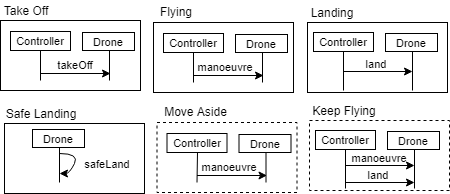
\includegraphics[width=\columnwidth]{figures/new_drone_bmsc.png}
%    \caption{bMSCs for the drone delivery scenario}
%    \label{fig:drone_bmsc}
%    \vspace*{-0.5cm}
%\end{figure}
% To move into implementation section

%We have developed LoTuS, an integrated development environment that supports the modeling of the extended hMSC, for what-if scenario analysis.
%Figure~\ref{fig:lotus} displays a screenshot when a tool is being used to create the model in Figure~\ref{fig:hmsc}.

%\begin{figure*}
% 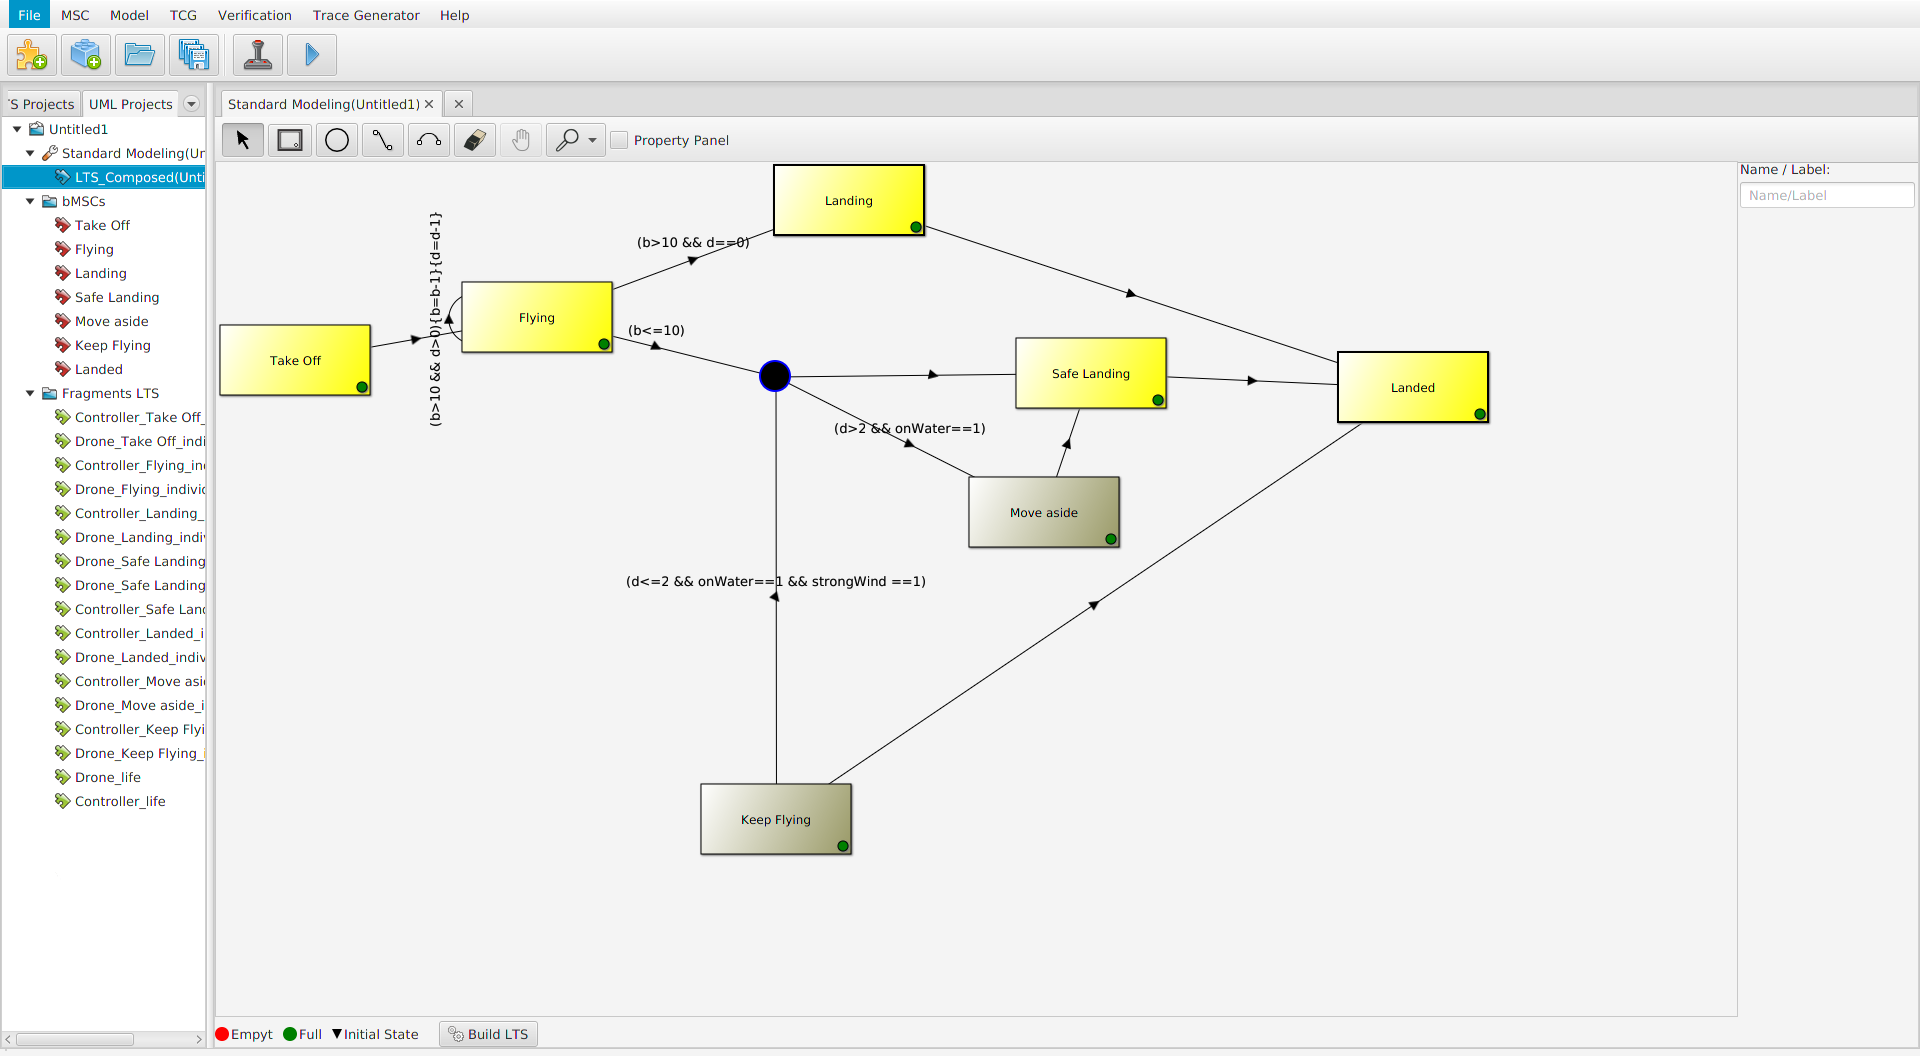
\includegraphics[width=0.8\textwidth]{figures/2-LoTuS.png}
%    \caption{LoTus: an IDE for modeling the extended MSCs. The project explore navigation view on the left shows the specification of individual bMSCs. }
%    \label{fig:lotus}
%    \vspace*{-0.25cm}
%\end{figure*}


%==========================


\subsection{The Wrapper Aspect}
The introduction of a {\it wrapper} $w(c)$ changes the defiant behaviour of the component $c$, i.e. $W_s, S_{w(c)} \not \models R_c$, retaining the essential satisfaction of global requirements when $c$ is substituted with $w(c)$:  $W_s, S'_s \models R_s$ where $S'_s = S_s |_{c \rightarrow w(c)}$. Furthermore, the adaptation is {\it cautious} because other than the exceptional condition $W_s$, the wrapped component should still behave like the original designed component, i.e., $(W_c \setminus W_s), S_{w(c)} \models R_c$. 

%\subsubsection{A Wrapper by Aspect-Orientation}
Based on aspect-oriented programming (AOP)~\cite{Kiczales:2001}, we introduce wrappers that can achieve the above requirements. The exceptional conditions identified in the scenarios provide an indication where changes in the system should occur ({\it joint points}). Once the join points are identified, we represent them as regular expressions as {\it point-cuts}, so that a replacement of the behaviour after the join points can be done through aspect {\it advices}. Aspect advices are exceptionally handled, which can invoke existing functionalities of original components, but can also introduce additional functions and conditions that do not exist in the original components.

%Since a component at design time is unaware of its future exceptional usage, it will not be able to expose its full implementation to the system integrator. Fortunately, {\it aspect-oriented} framework can intercept the control flow of the behavioural specification~\cite{Xu07}. 

%For example, to identify the join points, i.e., where  modifications are allowed to change. Methodologically, the exceptional conditions we obtain from the exceptional scenarios provide us a clue where such join points can be.

%Once the join points are identified, we can use regular expressions to express them as {\it point-cuts} so that a replacement of the behaviour after the join points can be done through aspect {\it advices}. Aspect advices in this situation are exceptional handling which can still invoke existing functionality of the original components, but can also introduce additional functions and conditions that do not exist in the original component. But the weaving of the aspect-oriented wrapper must be performed with caution. 

In the situation in which there are more than one wrapper for the same exceptional condition, to avoid interference~\cite{Katz:2008:IAI:1394496.1394500}, we define a precedence order among wrappers. For example, a safety wrapper is regarded with a high-level of importance and should be applied afterwards, to override applied unsafe wrappers. 

